\usetikzlibrary{arrows}
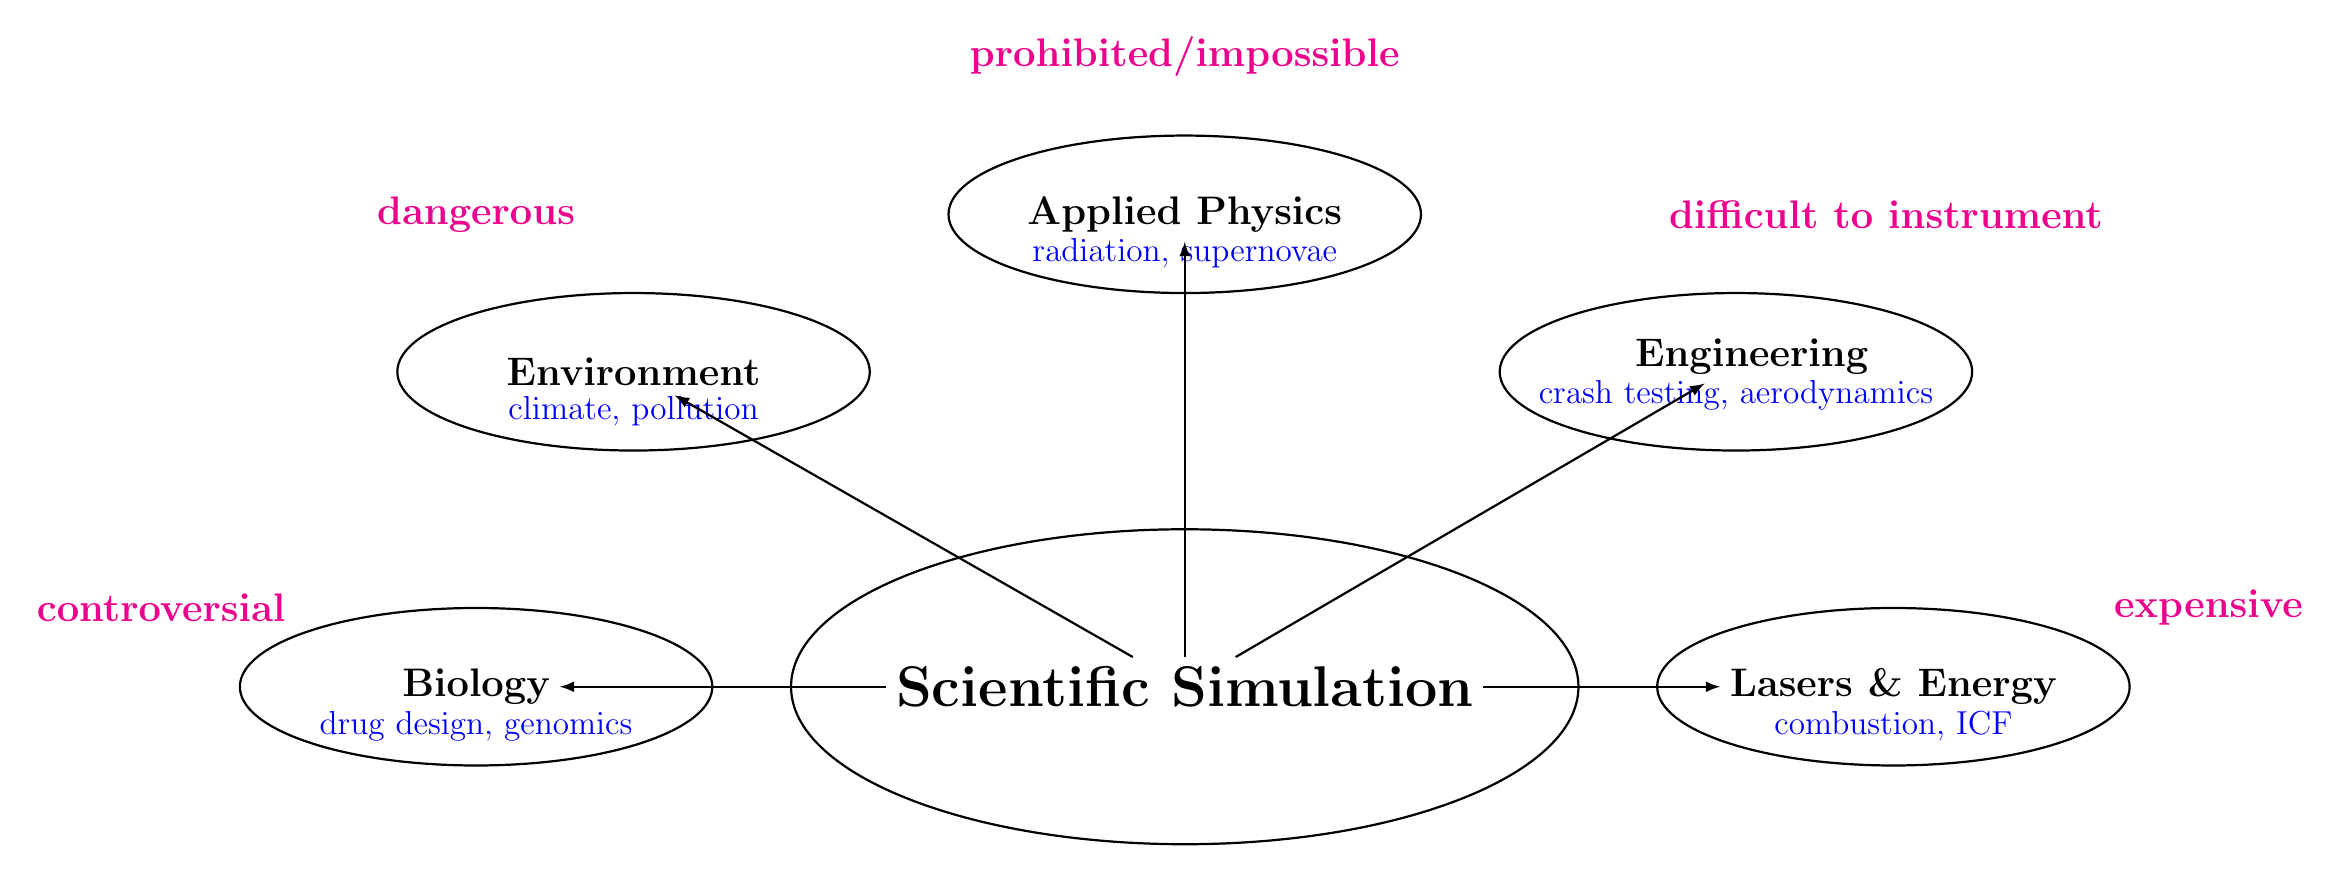
\begin{tikzpicture}

\draw[thick]  (-2,-1) ellipse (5 and 2);
\node (v1) at (-2,-1) {\huge \bf Scientific Simulation};

\draw[thick]  (-11,-1) ellipse (3 and 1);


\draw[thick]  (-9,3) ellipse (3 and 1);

\draw[thick]  (-2,5) ellipse (3 and 1);

\draw[thick]  (5,3) ellipse (3 and 1);

\draw[thick]  (7,-1) ellipse (3 and 1);

\node (v2) at (-11,-1) {\Large \bf Biology};
\node at (-11,-1.5) {\large \textcolor{blue}{drug design, genomics} };

\node (v3) at (-9,3) {\Large \bf Environment};
\node at (-9,2.5) {\large \textcolor{blue}{climate, pollution} };

\node (v4) at (-2,5) {\Large \bf Applied Physics};
\node at (-2,4.5) {\large \textcolor{blue}{radiation, supernovae} };

\node (v5) at (5.2,3.2) {\Large \bf Engineering};
\node at (5,2.7) {\large \textcolor{blue}{crash testing, aerodynamics} };

\node (v6) at (7,-1) {\Large \bf Lasers \& Energy};
\node at (7,-1.5) {\large \textcolor{blue}{combustion, ICF} };

\draw [thick, -latex] (v1) edge (v2);
\draw [thick, -latex] (v1) edge (v3);
\draw [thick, -latex] (v1) edge (v4);
\draw [thick, -latex] (v1) edge (v5);
\draw [thick, -latex] (v1) edge (v6);



\node at (-15,0) {\Large \bf \textcolor{magenta}{controversial}};
\node at (-11,5) {\Large \bf \textcolor{magenta}{dangerous}};
\node at (-2,7) {\Large \bf \textcolor{magenta}{prohibited/impossible}};
\node at (7,5) {\Large \bf \textcolor{magenta}{ difficult to instrument }};
\node at (11,0) {\Large \bf \textcolor{magenta}{expensive}};

\end{tikzpicture}